\chapter{Fundamentals Old}
\label{cha:Fundamentals Old}

This chapter provides an overview of foundational concepts relevant to the thesis. It begins by reviewing various positioning methods for indoor and outdoor settings, followed by an examination of how smartphones handle alerts, including different types and influencing factors in iOS. Geofencing technologies are analyzed for their functionality, use cases and limitations. Finally, advancements in technologies such as speech-to-text and large language models are discussed in the context of voice-controlled reminder systems.

\section{Positioning}
Positioning techniques are organized by the methods used to determine a location, with each approach offering specific benefits depending on the environment and application. The sections below introduce the core positioning methods developed over recent decades, including satellite-based positioning, cellular and WLAN-based positioning, proximity sensing, lateration and angulation. Each method has different principles for calculating location, whether through signal timing, distance, or angle measurements. The following sections will explore the fundamental concepts behind each technique, detailing how they calculate a position and discussing the advantages and limitations that make each method suitable for different scenarios.

\subsection{Cellular or WLAN Positioning}
Cellular and WLAN positioning are two different methods used to determine a device's location, especially when GPS is unavailable or needs to be supplemented. Cellular positioning relies on signals from nearby cell towers, using trilateration or multilateration techniques to calculate the device's distance from each tower. These techniques calculate position by measuring signal travel times or signal strength to multiple towers, which enables a triangulated location, as discussed by K\"upper \cite{kupper2005location}. This method is particularly effective in rural areas where WLAN networks may be sparse, though the accuracy decreases in low-density tower areas due to the increased distances between towers.
Meanwhile, Kolodziej and Hjelm \cite{kolodziej2017local} highlight that WLAN positioning estimates a device's location by analyzing signals from nearby access points. For this approach, a database or map of known WLAN access points with their geographic locations is necessary in order to compare signal strengths and determine relative proximity. K\"upper \cite{kupper2005location} states that because of signal variability indoors, WLAN positioning often works best in urban or indoor environments where multiple access points are available for cross-referencing.

\subsection{Proximity Sensing}
Proximity sensing estimates a device's location by assessing signal interactions with nearby known transmitters, such as access points, beacons, or other devices. Depending on the infrastructure available, it can either use cellular or WLAN networks. As K\"upper \cite{kupper2005location} notes, proximity sensing achieves high accuracy in locations with a high concentration of access points, such as indoor environments like malls and airports where WLAN is widely available.
Outdoors, however, accuracy can vary significantly due to the reduced availability of proximity devices. Indoors, proximity sensors such as WLAN or Bluetooth beacons can achieve precision within a range of a few meters. Though this method provides great accuracy, a continuous connection to nearby beacons is required, resulting in high power consumption. Furthermore, it can sometimes cause delays in applications due to its reliance on the quality and consistency of signal strength, according to Mautz \cite{mautz2012indoor}.
Proximity sensing methods are frequently combined with other positioning systems like GPS or inertial motion sensors to form stronger and more accurate hybrid systems. This combination improves both reliability and precision across diverse environments. In outdoor settings, GPS is often used as the primary source, with proximity sensing employed as a secondary technique. In the words of K\"upper \cite{kupper2005location}, proximity sensing in cellular networks is often referred to as Cell of Origin (CoO), Cell Global Identity (CGI), or Cell-ID and while it has reduced accuracy in both, cellular and WLAN networks, it is the easiest to implement.

\subsection{Cell of Origin}
Cell of Origin (CoO) is a basic mobile positioning technique used to identify the specific cell in which a device or caller is located. A "cell" is a geographic area within the cellular network, managed by a base station (BS), which serves as a local signal hub for devices within that area. The accuracy of the location determined through CoO depends largely on the size and shape of the cell, as highlighted by Grejner-Brzezinska and Kealy \cite{grejner2004positioning}. Smaller cells result in a more precise position, often reaching accuracy within 100 meters in urban areas where cell towers are densely placed. In rural areas, cell coverage may span several kilometers, reducing CoO accuracy.

Each cell may contain multiple overlapping service areas, meaning a device or mobile station (MS) could be within the range of multiple base stations, allowing it to detect and communicate with several base station IDs simultaneously. According to Jan, Chu et al. \cite{jan2004improving}, an MS located in region A can receive signals from BSs 0, 1 and 6; in region B, it might connect to BSs 0 and 2; and in region C, it may only detect signals from BS 0. The area where a MS detects a unique combination of base station signals is called a localization region. For example, the cell of BS 0 contains 13 distinct localization regions (A-M).
These corresponding localization regions are linked to specific sets of base station IDs in a centralized table or database, which is managed by a server. When a MS reports receiving signals from specific BSs, the server consults this table to determine the MS's location. For instance, if the MS detects signals from BSs 0, 1 and 6, the server can identify that the device is located in region A, allowing for accurate localization of the MS's position, as stated by Jan, Chu et al. \cite{jan2004improving}. This configuration is demonstrated in Fig.~\ref{fig:coo}.

\begin{figure}[htbp]
    \centering
    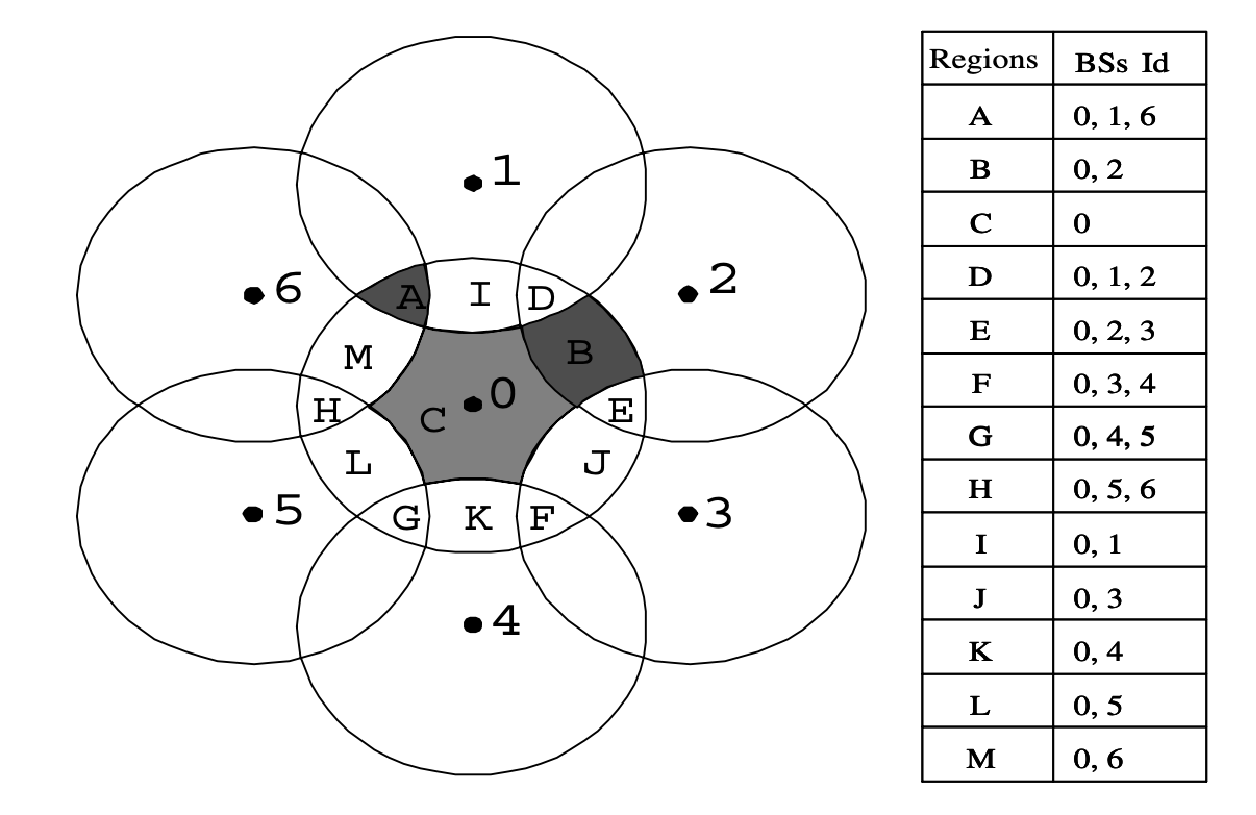
\includegraphics[width=0.7\textwidth]{COO.pdf}
    \caption{A layout of the cell-based positioning network \cite{jan2004improving}}
    \label{fig:coo}
\end{figure}

CoO is often used in scenarios where approximate location data is sufficient. It's commonly used in emergency services to approximate a caller's location or for network optimization by telecom providers. Per Grejner-Brzezinska and Kealy \cite{grejner2004positioning}, CoO is a power-efficient solution, as it only requires a single connection to the cell tower, making it accessible across cellular networks, even in low-power settings where more intensive GPS tracking might be impossible.

\subsection{Lateration}
Lateration calculates a target's location by using distance or distance differences from multiple reference stations, typically requiring at least three to achieve accuracy. These measurements, often referred to as "pseudoranges" due to inevitable errors, are based on the signal strength loss experienced by the beacon as it travels between the target and access points. Lateration techniques are categorized into circular lateration, which relies on absolute distance measurements and hyperbolic lateration, which uses differences in these distances across stations.

\subsubsection{Circular Lateration}
Circular lateration is a method used in positioning systems to determine a target's location by measuring distances to multiple base stations. Assuming the base stations are at the same elevation, knowing the distance between the target and a single base station places the target somewhere on a circle centered on that station. Introducing a second base station allows for two possible positions where the two circles intersect. Adding a third base station resolves this uncertainty, pinpointing the target's exact location at the single intersection point of all three circles, according to K\"upper \cite{kupper2005location}. This process, known as trilateration, utilizes the Pythagorean theorem for calculations and is illustrated in Fig.~\ref{fig:circular_lateration}.

\begin{figure}[htbp]
    \centering
    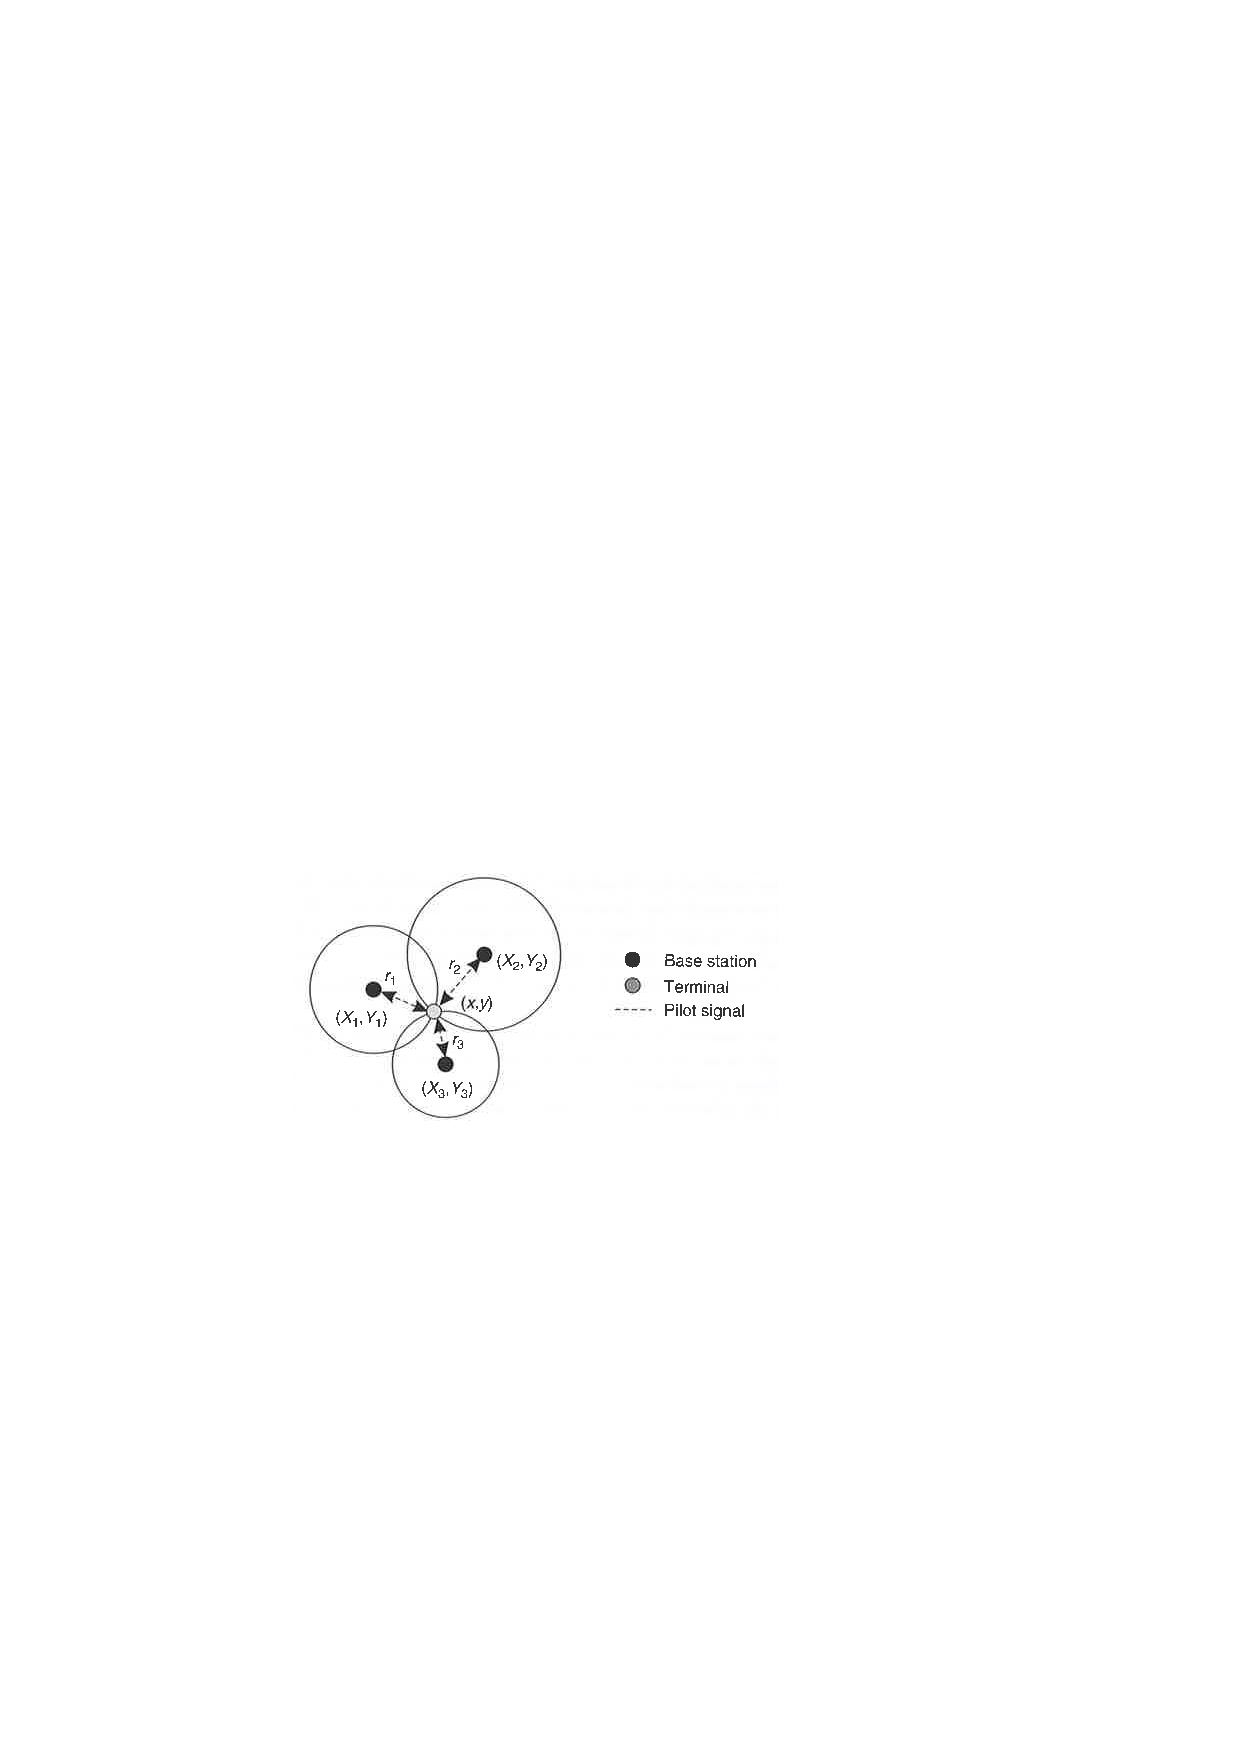
\includegraphics[width=0.7\textwidth]{circular_lateration.pdf}
    \caption{2D Circular lateration with three base stations \cite{kupper2005location}}
    \label{fig:circular_lateration}
\end{figure}

In three-dimensional space, each distance measurement defines a sphere around a base station. Kolodziej and Hjelm \cite{kolodziej2017local} note that with only three base stations, the target's position is narrowed down to two possible points where the spheres intersect. Typically, one of these points can be dismissed as implausible, such as a location in outer space. To eliminate any ambiguity, a fourth base station is introduced, ensuring a unique position fix. Additionally, the fourth base station aids in synchronizing clocks, enhancing the accuracy of the positioning system.

\subsubsection{Hyperbolic Lateration}
In contrast to circular lateration, hyperbolic lateration determines a position by measuring differences in distance rather than absolute distances. A hyperbola represents all points that maintain a constant range difference relative to two fixed points, typically two base stations. K\"upper \cite{kupper2005location} explains that with the known range difference between the target and two base stations, the target's possible locations are constrained along a hyperbolic path between them. This method, illustrated in part (a) of Fig.~\ref{fig:hyperbolic_lateration}, uses two base stations to determine a single hyperbolic path. However, with just two base stations, the target's precise location cannot be unambiguously determined, as it could lie anywhere along the hyperbola.
To resolve this ambiguity, a third base station is introduced, as shown in (b). By adding this third base station, a second hyperbola is created and the target's position is estimated at the intersection of these two hyperbolas. In three-dimensional space, the principle extends to hyperboloids, requiring at least three base stations for an unambiguous position fix. A key advantage of hyperbolic lateration is that it only requires synchronization among the base stations' clocks, rather than between the stations and the target, simplifying timing coordination.

\begin{figure}[htbp]
    \centering
    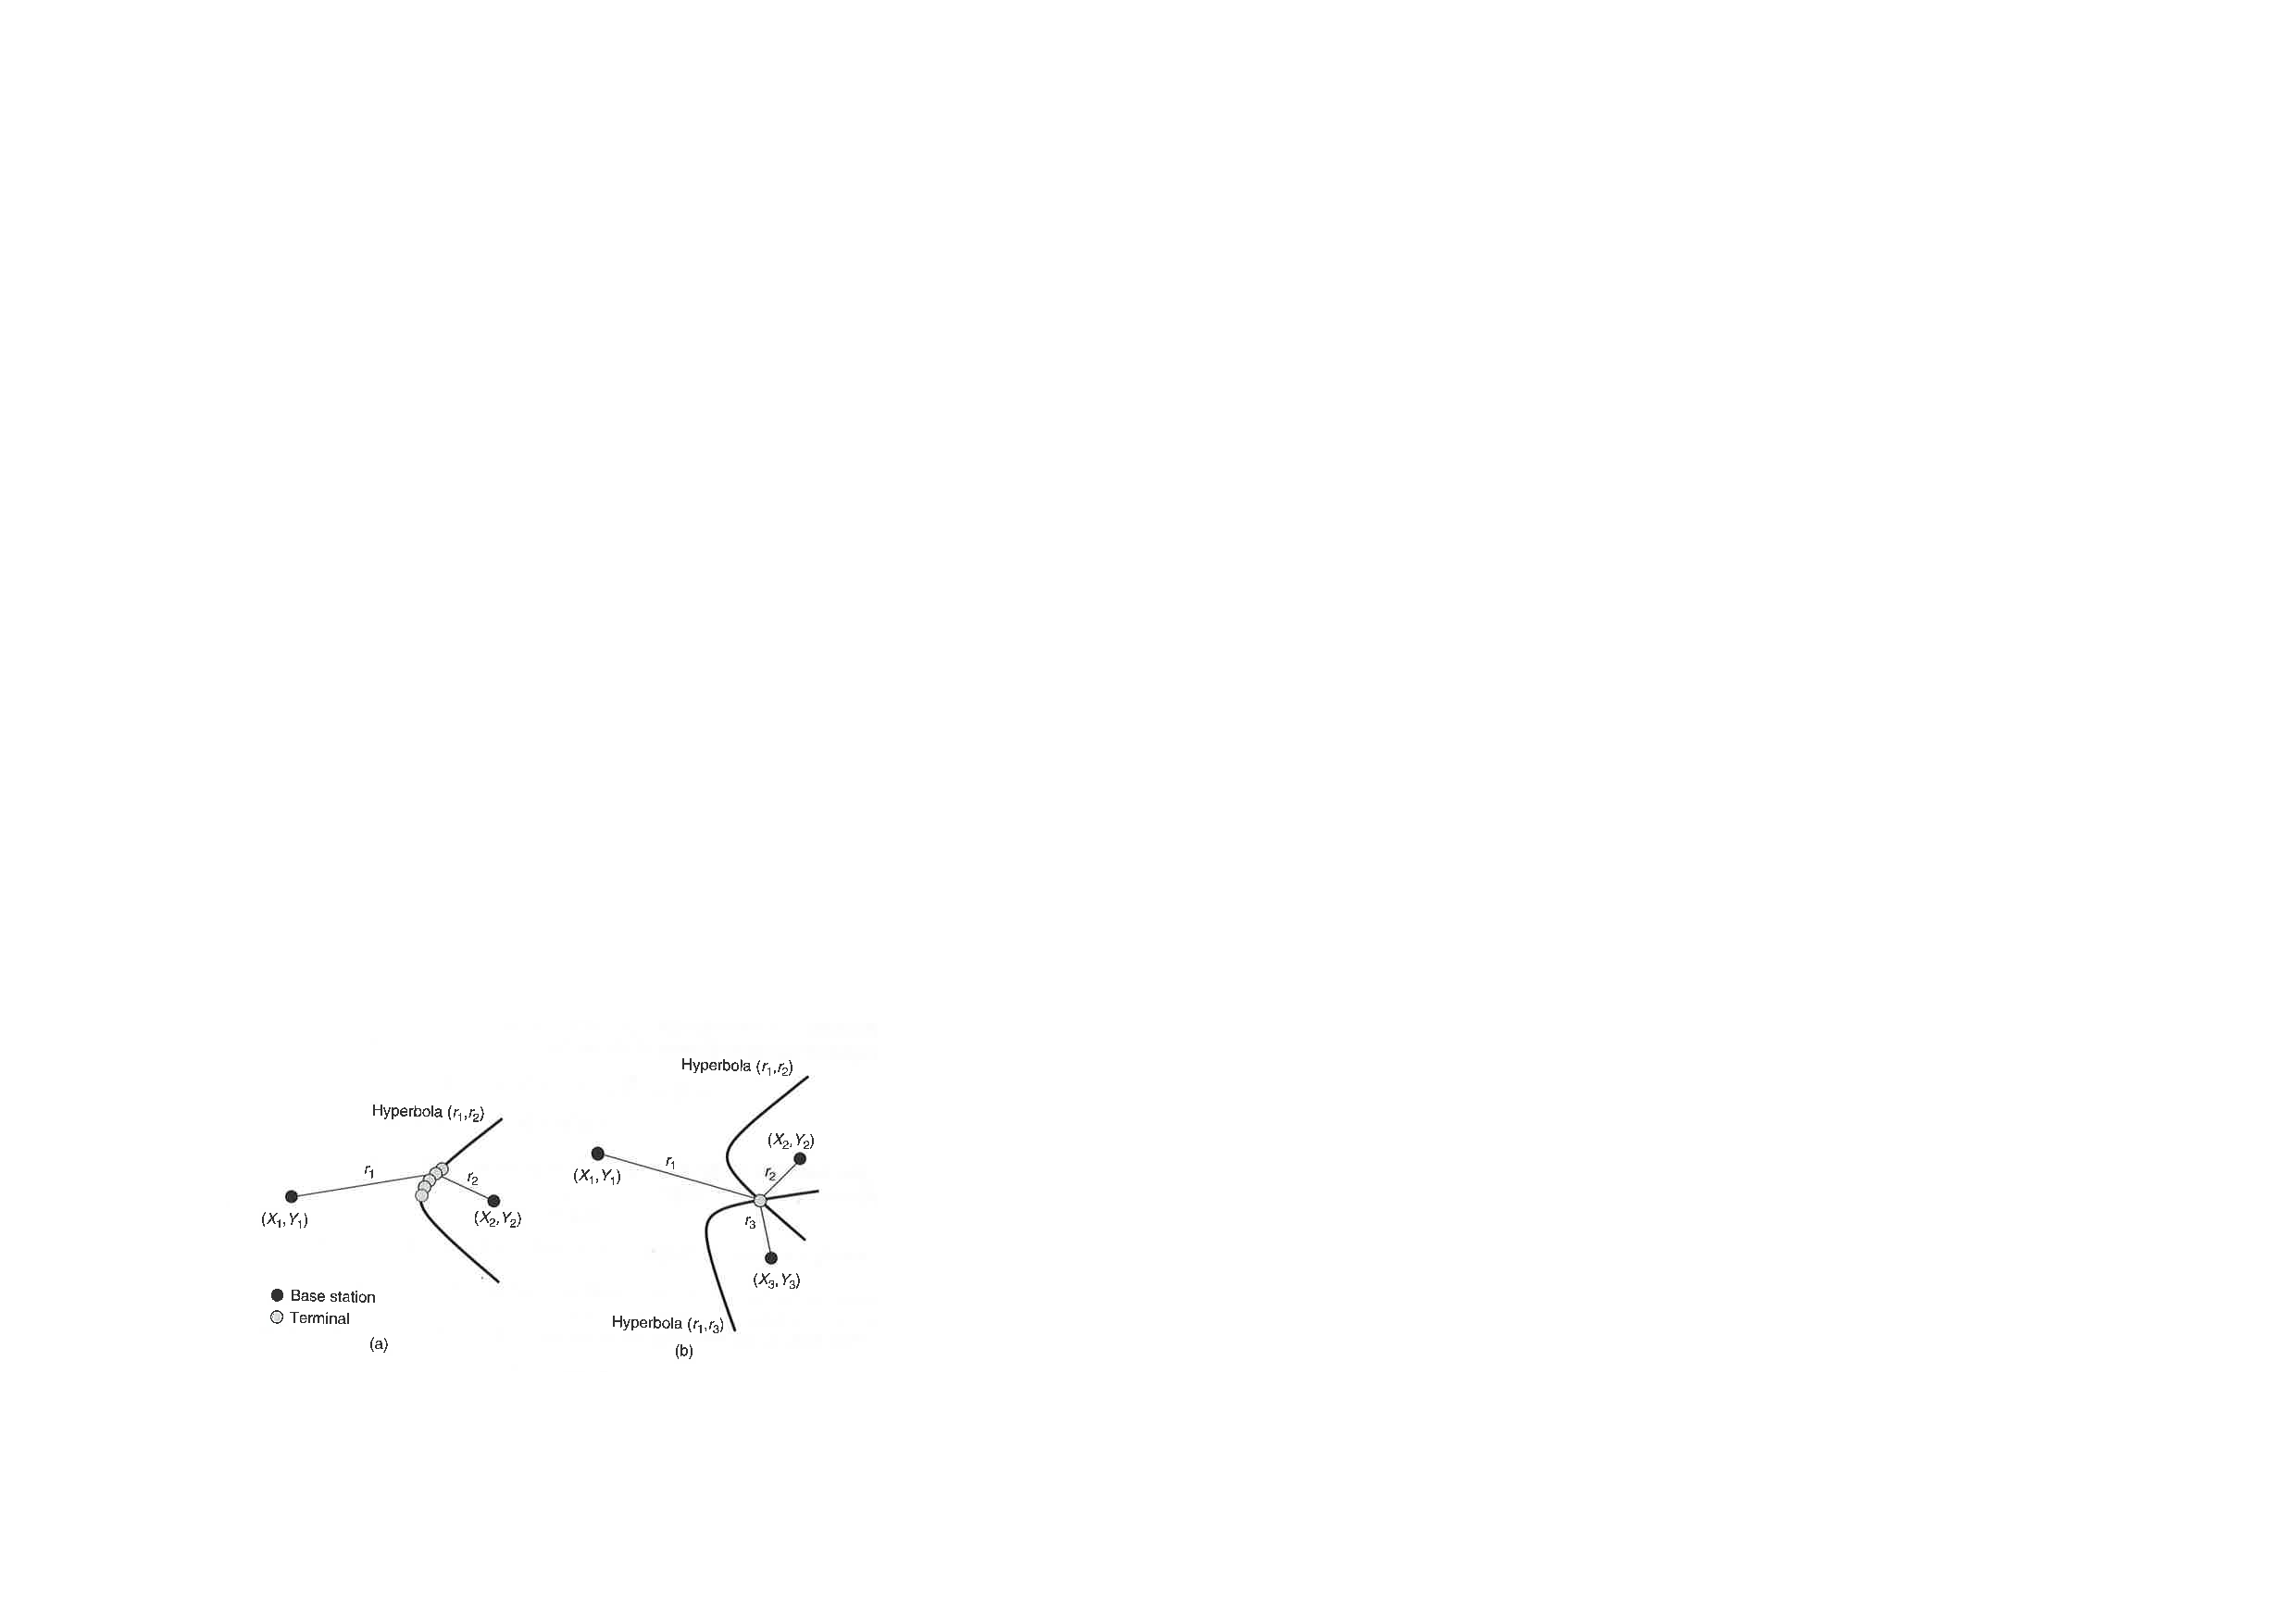
\includegraphics[width=0.7\textwidth]{hyperbolic_lateration.pdf}
    \caption{Hyperbolic lateration with two (a) and three (b) base stations \cite{kupper2005location}}
    \label{fig:hyperbolic_lateration}
\end{figure}

\subsection{Angulation}
Angulation is a positioning technique that determines an object's location based on the angles at which signals are received from multiple reference points, rather than measuring distances. According to K\"upper \cite{kupper2005location} it is also called Angle of Arrival (AoA) or Direction of Arrival (DoA). Werner \cite{werner2014indoor} explains that by using directional antennas or other angle-measuring equipment, the system identifies the direction of incoming signals from known base stations or access points. Once the angles from at least two base stations are known, the object's position can be triangulated by drawing lines along these angles, the point where the lines intersect reveals the target's location, as shown in Fig.~\ref{fig:angulation}.

\begin{figure}[htbp]
    \centering
    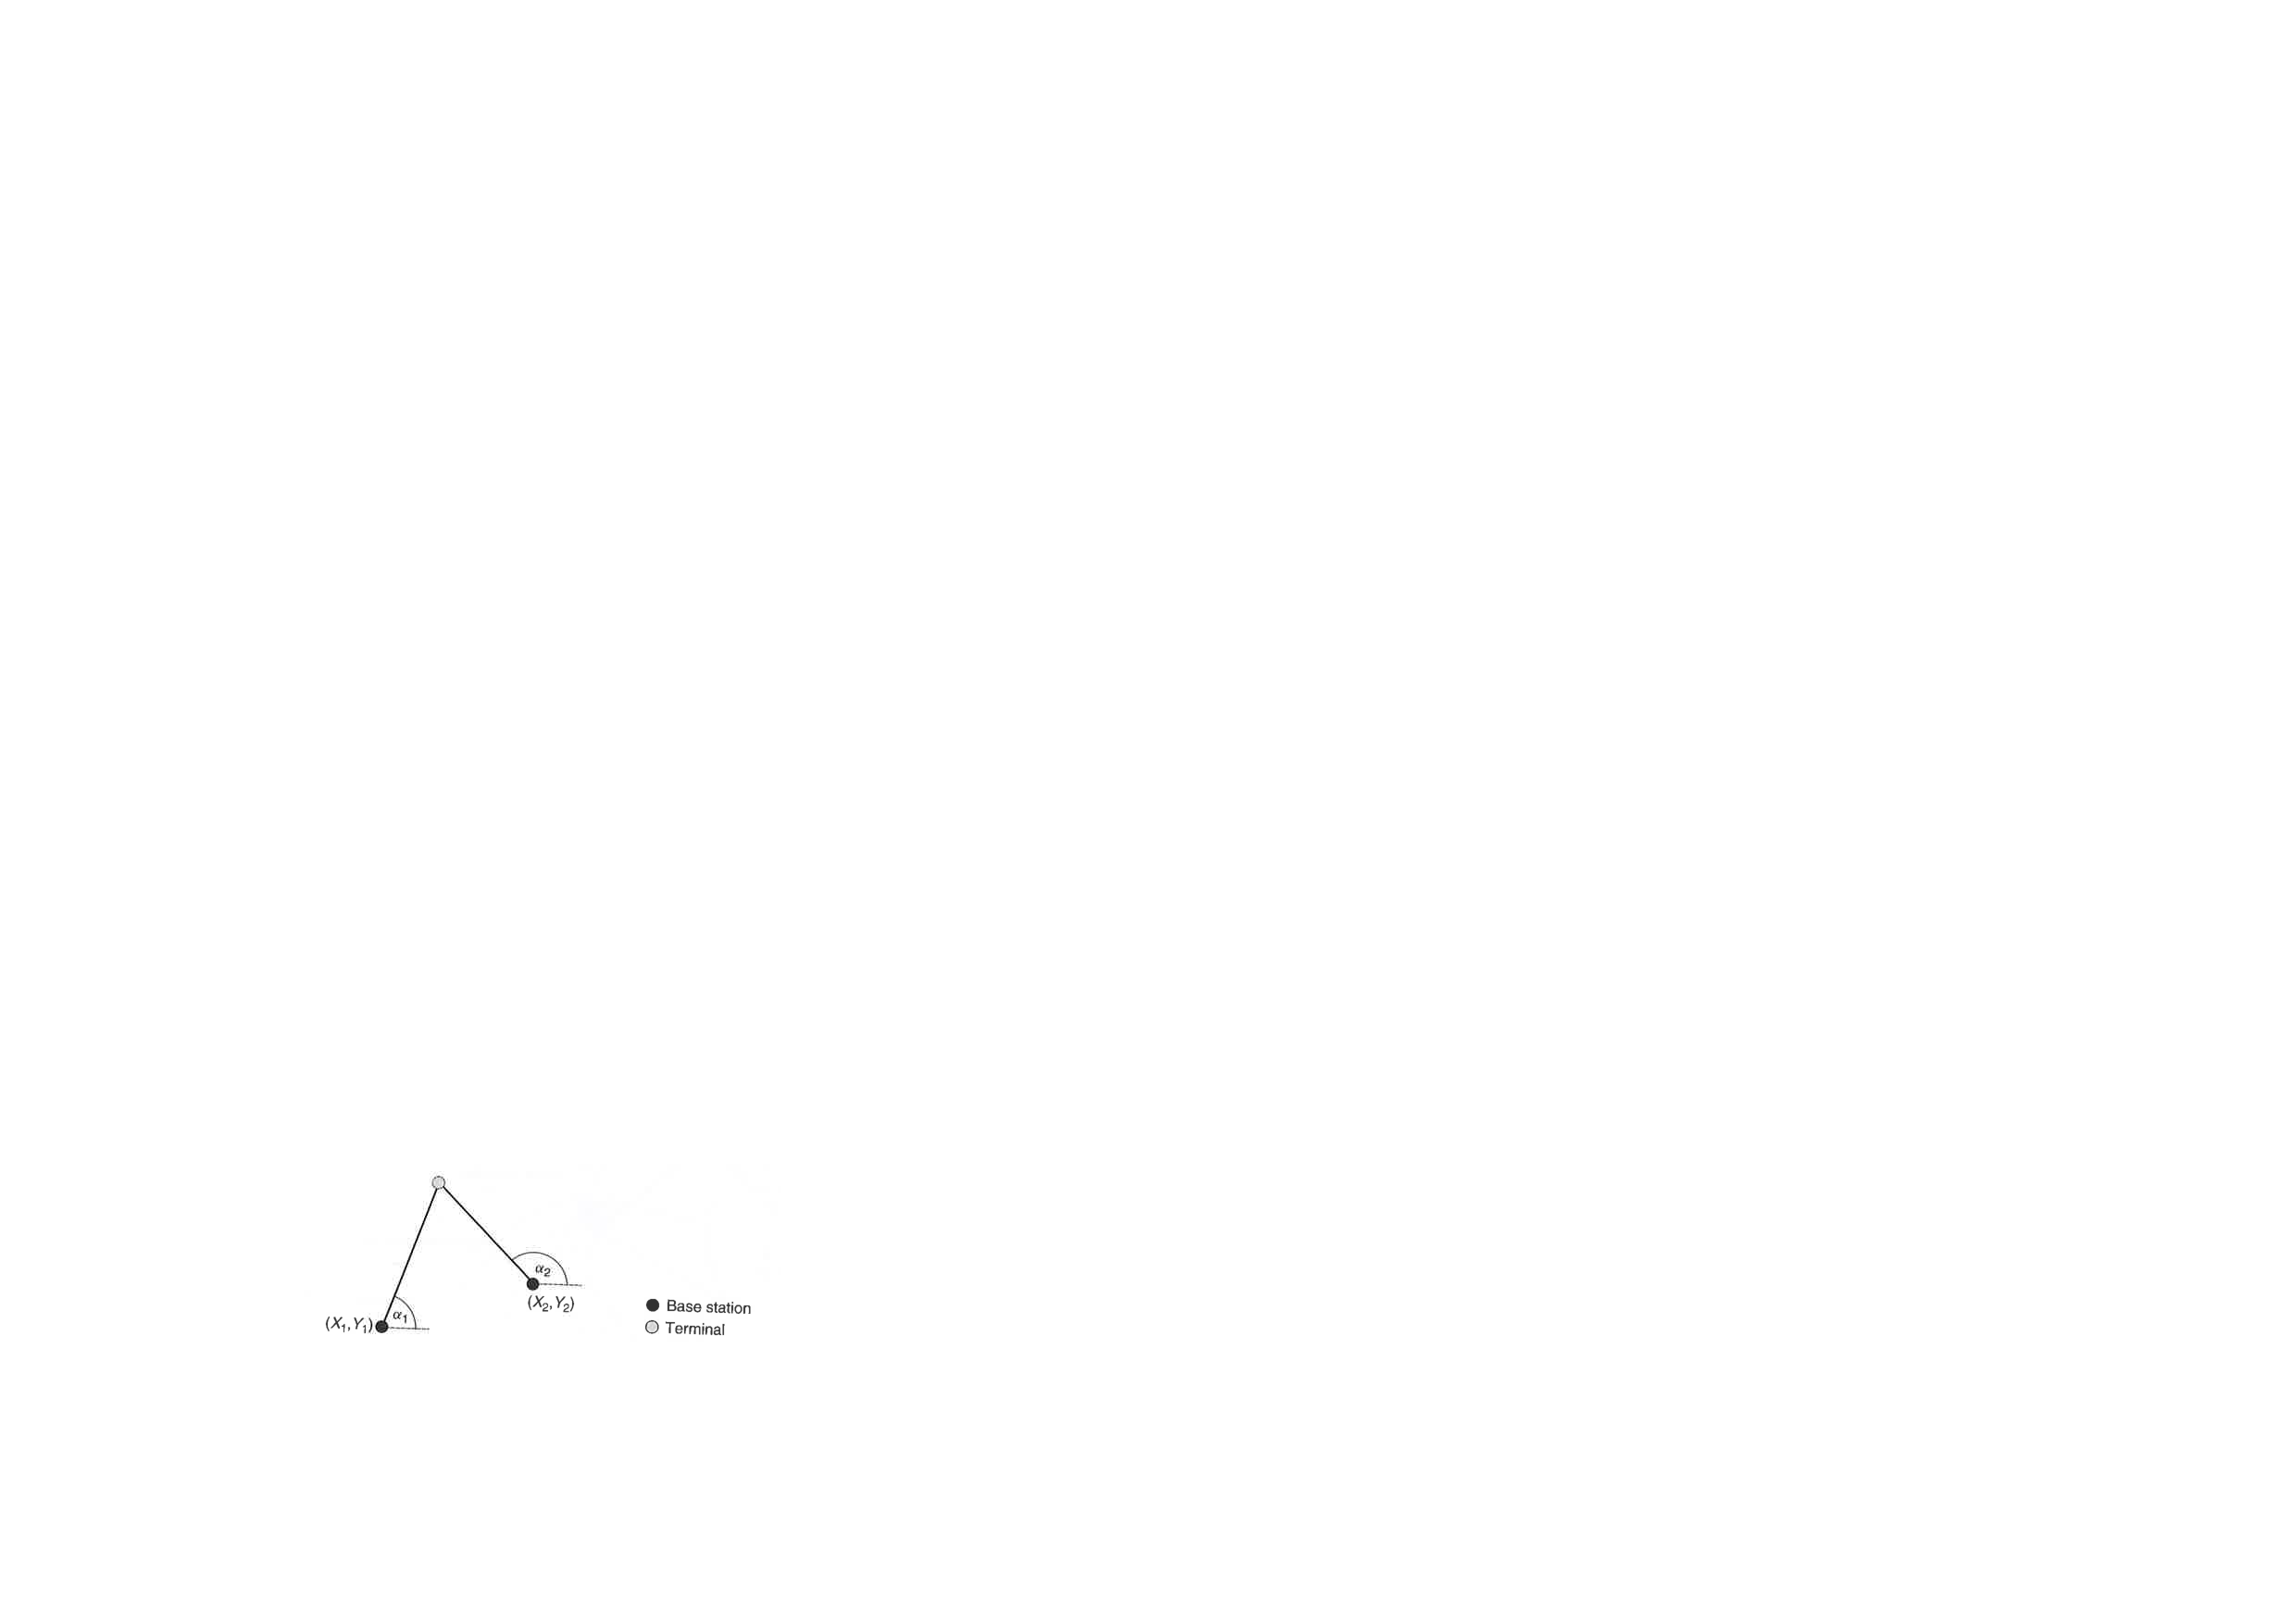
\includegraphics[width=0.7\textwidth]{angulation.pdf}
    \caption{Angulation with two base stations \cite{kupper2005location}}
    \label{fig:angulation}
\end{figure}

In three-dimensional space, a third angle may be required for accurate positioning. Angulation offers an effective alternative to lateration methods, particularly in environments where measuring precise distances is challenging due to signal reflections or interference. However, it does require precise angle measurements, which can be sensitive to minor errors in directionality, especially at long distances.

\subsection{GNSS}
The Global Navigation Satellite System (GNSS) is an international network of satellites providing real-time positioning and timing data to various users worldwide. Originally developed to meet the demands for precise global navigation, GNSS aims to deliver accurate and reliable positioning for civil, commercial and scientific applications beyond military uses. GNSS systems, such as GPS (USA), GLONASS (Russia), Galileo (EU) and BeiDou (China), share a basic structure that includes space, control and user segments. Kaplan and Hegarty \cite{kaplan2017understanding} highlight that the space segment consists of a constellation of satellites orbiting Earth. The control segment ensures that ground stations monitor the satellites and adjust their paths if needed. The user segment, however, says that users can access signals from at least four satellites at any given time in order to calculate an accurate 3D position through trilateration.
GNSS satellites transmit signals containing information about their location and timing, allowing receivers on the ground to determine distance by calculating the time delay in signal arrival, which is known as time-of-arrival positioning, as stated by Enge \cite{enge1994global}. High-accuracy GNSS is achieved with systems like Differential GNSS (DGPS), which uses reference stations on the ground to correct errors from atmospheric interference, satellite orbit irregularities and clock discrepancies.

%---------------------------------------------------------------------------------------------------------------------------------------------------------------------------------------------------------------------------------------------------------------------------------------------------------------------------------------------------------------------------------

\section{Alerts on Smartphones}
Alert types, trigger conditions and restrictions define how and when users are notified of specific app events, ensuring that alerts provide value without disrupting user control or device functionality. The following sections outline the types of alerts available, the mechanisms that trigger them and the specific guidelines imposed by Apple to maintain a responsible alert experience to users.

\subsection{Alert Types}
Smartphones provide users with various alert mechanisms, ranging from visual and auditory cues to haptic feedback. These feedback types are important for confirming actions, delivering critical information, or enhancing user experience. Notifications are among the most widely used feedback types and they can be divided into local and push notifications. According to Apple's documentation \cite{apple_local_notifications}\cite{apple_push_notifications}, local notifications are generated by the app itself to inform users of important events or reminders, even when the app is running in the background, while push notifications are server-sent, commonly used for real-time updates such as messaging notifications or breaking news alerts.
Another significant alert type is haptic feedback, which alerts the user physically through vibrations. In iOS, the primary tools for haptic feedback include the UIImpactFeedbackGenerator, which provides feedback for different levels of physical impact, such as light, medium, or heavy taps. 
The UISelectionFeedbackGenerator is used to indicate changes in selection, such as scrolling through options in a picker and lastly the UINotificationFeedbackGenerator conveys success, warning, or error notifications to enhance the clarity of critical feedback, as highlighted by the Apple Dev-Pages \cite{apple_haptics}.
In addition to haptics, sound feedback is available, which is more noticeable but also more effective in capturing users' attention. As per Apple's guidelines \cite{apple_sound_guidelines}, sounds in iOS are divided into system sounds, which are used for standard actions like errors or confirmations and custom sounds, which are often used in games or specific app events, providing unique auditory experiences. 
For visual feedback, Apple's UIAlertController \cite{apple_alerts} offers pop-up alerts with titles, messages and action buttons and is commonly used for critical alerts or confirmations, providing a controlled interruption compared to sounds.
Toasts are non-intrusive messages that appear briefly and disappear without needing user interaction. While they aren't native to iOS, third-party frameworks can enable them, offering a less intrusive way to communicate short information. Subtler forms of visual feedback, such as progress indicators and badges, are also effective for showing ongoing tasks or indicating unread notifications within app sections. 
With iOS 16, Apple introduced the Live Activities feature \cite{apple_live_activities}, which can be used to display real-time updates on the lock screen or in the Dynamic Island. This feature allows users to stay informed about ongoing events, such as tracking a food delivery or monitoring live sports scores, without needing to open the app.

\subsection{Triggers}
In iOS, alerts aren't only triggered by user input, they can also be set off by automated and event-based conditions. For instance, apps can use scheduled timers to trigger alerts or notifications at specific times, like for reminders, countdowns, or regular updates, easily implemented with Swift's Timer class \cite{apple_timer}.
Additionally, alerts can be triggered based on app state changes, such as entering the background, coming to the foreground, or closing. For example, an app may display a confirmation alert when the user tries to leave a page with unsaved data or notify them of an important update using UIApplicationDelegate \cite{apple_app_delegate}.
Device sensors, like the accelerometer and gyroscope, can detect movement or orientation changes and trigger alerts accordingly. As noted by Apple \cite{apple_corelocation}\cite{apple_coremotion}, location-based triggers can also activate alerts or notifications when the user enters or exits a specific region, which is a key point in this thesis. For this purpose, CLLocationManager is useful for handling location-based triggers, while CoreMotion supports detecting motion events. Additionally, Apple's HealthKit \cite{apple_healthkit} allows apps to create alerts based on user health data. For example, a notification can be sent if a user's heart rate exceeds a certain threshold.
To manage in-app alerts, Apple \cite{apple_notificationcenter} recommends using NotificationCenter is often used to broadcast data changes so that observers can display alerts or badges when specific data updates. For notifications, iOS provides three main trigger types. UNTimeIntervalNotificationTrigger \cite{apple_time_trigger} schedules a notification after a set time interval, while UNCalendarNotificationTrigger \cite{apple_calender_trigger} delivers notifications at specific dates and times, either once or repeatedly. Most relevant to this thesis is UNLocationNotificationTrigger \cite{apple_location_trigger}, which sends notifications when the user enters or exits a designated geographical area.

\subsection{Restrictions in iOS}
When it comes to responsible app development, Apple has many guidelines to maintain user control, ensure privacy and prevent disruptive app behavior. Generally, apps are restricted from triggering alarms or alerts when they are not actively running in the foreground, with exceptions for specific cases like VoIP (Voice over IP), music streaming and location-tracking apps. These apps can run background audio, but this is not intended for alarms and comes with strict guidelines to prevent misuse. For instance, per Apple's guidelines \cite{apple_background_audio_guidelines}, while a music app may play in the background, an alarm app that tries to exploit this mode to ring an alarm would be rejected. This limitation makes it challenging to release an app that plays sounds solely for alerts, though this is not the goal of this thesis.
Additionally, iOS does not provide any public API for third-party apps to set, modify, or access alarms in the native Clock app, which is entirely separate and inaccessible for tasks like scheduling alarms or timers.
When delivering notifications, apps must obtain user permission. Users can choose to allow, mute, or disable notifications from each app and Apple discourages excessive notifications, especially those lacking immediate or relevant value. Apps that send spammy notifications risk penalties or even removal from the App Store. Custom sounds for local notifications are limited to 30 seconds, if a sound exceeds this limit, iOS defaults to the standard notification sound, as discussed on the Apple Developer website \cite{apple_sound_guidelines}. Local notifications also respect Silent Mode and Do Not Disturb settings, meaning sounds will not play if these modes are active. According to Apple's documentation \cite{apple_critical_alerts} critical alerts are allowed to bypass these settings, but this permission is reserved for essential use cases, such as health monitoring or emergency alerts, not for general alarms or reminders.
Location-based triggers, such as geofencing, also require explicit user permission. iOS limits the frequency of location-based notifications and may throttle frequent triggers. Excessive location tracking can lead to App Store rejection unless it is essential to the app's function. Additionally, Apple \cite{apple_geofencing_limits} restricts the use of geofencing to a maximum of 20 active geofences per app to conserve battery life and optimize performance.

\section{Geofencing}
Shevchenko and Reips \cite{shevchenko2024geofencing} define geofencing as the automated triggering of actions when "virtual boundaries around specific locations" are crossed. It relies on multiple location-based technologies, including GNSS, Wi-Fi, and cellular networks, to establish and monitor these predefined geographic boundaries. Over time, it has become a useful tool with applications across different industries.

Geofencing enhances user experiences by providing personalized services, such as sending targeted advertisements or adjusting smart home settings when people enter or leave specific areas. It is also widely used in business operations, including logistics, healthcare and workforce management, where it helps streamline processes and improve efficiency. However, as Greenwald \cite{greenwald2011geofencing} highlights, geofencing raises significant concerns, particularly regarding privacy. Since it relies on continuous location tracking, users' sensitive data may be vulnerable to misuse or security breaches, especially when the technology overlaps with personal or sensitive areas such as homes or healthcare facilities.

Initially designed for military and government use in the 1990s, geofencing has since expanded into a variety of domains due to advancements in GPS-enabled smartphones and mobile technologies \cite{westbrook2019gps}. In marketing, for instance, businesses use geofencing to send location-based advertisements or discounts to customers near their stores, creating personalized shopping experiences and increasing sales \cite{greenwald2011geofencing}. Workforce management benefits from geofencing by automating employee attendance tracking, where staff can clock in and out automatically upon entering or leaving work zones, reducing manual errors and administrative burdens \cite{amudha2019smarthome}.
Geofencing is also transforming home automation in the Internet of Things (IoT) domain. For example, smart devices can adjust lighting, heating, or security systems based on residents' proximity to their homes \cite{amudha2019smarthome}. Similarly, it has proven valuable in agriculture, where geofencing combined with IoT helps protect crops from wild animal intrusions by sending farmers real-time alerts to minimize damage \cite{kadam2020crops}. In educational settings, Takyiwa-Debrah \cite{takyiwa2023geofence} highlights how geofencing improves child safety by integrating GPS-enabled wearable devices, which provide real-time location tracking to prevent abductions in schools.
In logistics, geofencing ensures vehicles adhere to designated routes and allows businesses to monitor fleet locations in real time, improving efficiency and security \cite{reclus2009fleet}. In healthcare, it helps caregivers monitor dementia patients by setting up safe zones and alerting them when patients move beyond these boundaries, enabling prompt interventions and ensuring patient safety \cite{arora2023location}.

\section{Converting Speech to Text}
Speech-to-text (STT) is a technology that turns spoken words into written text. It works by listening to audio and using voice recognition to understand and transcribe the words. The result is a text document that captures what was said. While speaking is the most natural and efficient way to communicate, audio recordings alone can be difficult to review or reuse quickly. This makes speech-to-text an essential tool across many fields. For instance, it enables record-keeping of patient notes in healthcare or court proceedings in legal services, supports transcription of lectures in education, streamlines workflows in media and customer service by converting interviews or calls into text. Furthermore, it is widely used in virtual assistants to process voice commands, as well as in closed captioning to make videos accessible to broader audiences. It also plays a key role in creating accessibility tools for individuals with hearing impairments.

Rabiner and Juang \cite{rabiner1993speechrecognition} explain that speech can be understood as an audio signal characterized by its frequency, amplitude and temporal patterns, which define the unique qualities of spoken language. They further emphasize that speech is made up of different components that work together to create meaning and structure. One of the most basic elements is phonemes, which are the smallest units of sound in a language, like the "b" in "bat". These phonemes combine to form syllables, which are the building blocks of words, such as "bat" having one syllable and "better" having two. Beyond these, intonation patterns refer to the rise and fall of pitch in speech, which help convey emotions, emphasis or the difference between a question and a statement. According to Reetz \cite{reetz2020phonetics}, the process of turning speech into text depends on acoustic properties and linguistic understanding. Acoustic models focus on the sound itself, breaking down the audio into patterns like pitch, tone and duration to identify specific sounds or words. Meanwhile, language models go a step further by applying rules of grammar, vocabulary and sentence structure to make sense of those sounds in context. Together, these models ensure that the transcription is not only accurate in identifying the sounds but also meaningful and grammatically correct in written form.

However, speech-to-text faces several challenges that can impact its accuracy. Background noise, such as conversations, traffic or music, can interfere with speech clarity and make transcription difficult. Regional accents and dialects add variability in pronunciation, which can lead to misinterpretations. Additionally, Zechner and Waibel \cite{zechner20000spontaeousspeech} highlight that conversations with multiple speakers, especially when voices overlap, present difficulties in separating speech accurately. Spontaneous speech, with its non-standard grammar, fillers like "um" or "uh," and frequent self-corrections, further complicates transcription, as stated by Furiu et al. \cite{furiu2004spontaneousspeech}. Lastly, technical vocabulary can be challenging for the system to recognize without prior training.

In Fig.~\ref{fig:stt_pipeline} by Rabiner and Juang \cite{rabiner1993speechrecognition}  the speech-to-text pipeline is illustrated by breaking down the process into different stages, starting with signal processing, where speech is captured and analyzed to differentiate between voiced, unvoiced and silent segments. Next, feature extraction transforms the raw audio into meaningful data points, which are then segmented into smaller units for easier processing. The labeling and sound merging steps classify individual sounds and combine them into coherent units, guided by sound classification and phonotactic rules. Sound classification identifies sounds, such as vowels or consonants, based on their unique acoustic patterns, while phonotactic rules ensure that recognized sounds follow the natural language patterns, enhancing transcription accuracy.  Word verification and sentence verification ensure the transcription is contextually meaningful by leveraging lexical access and language models. Throughout the pipeline, knowledge sources such as phonotactic rules and linguistic models play an important role in improving the transcription and producing a recognized utterance.

\begin{figure}[htbp]
    \centering
    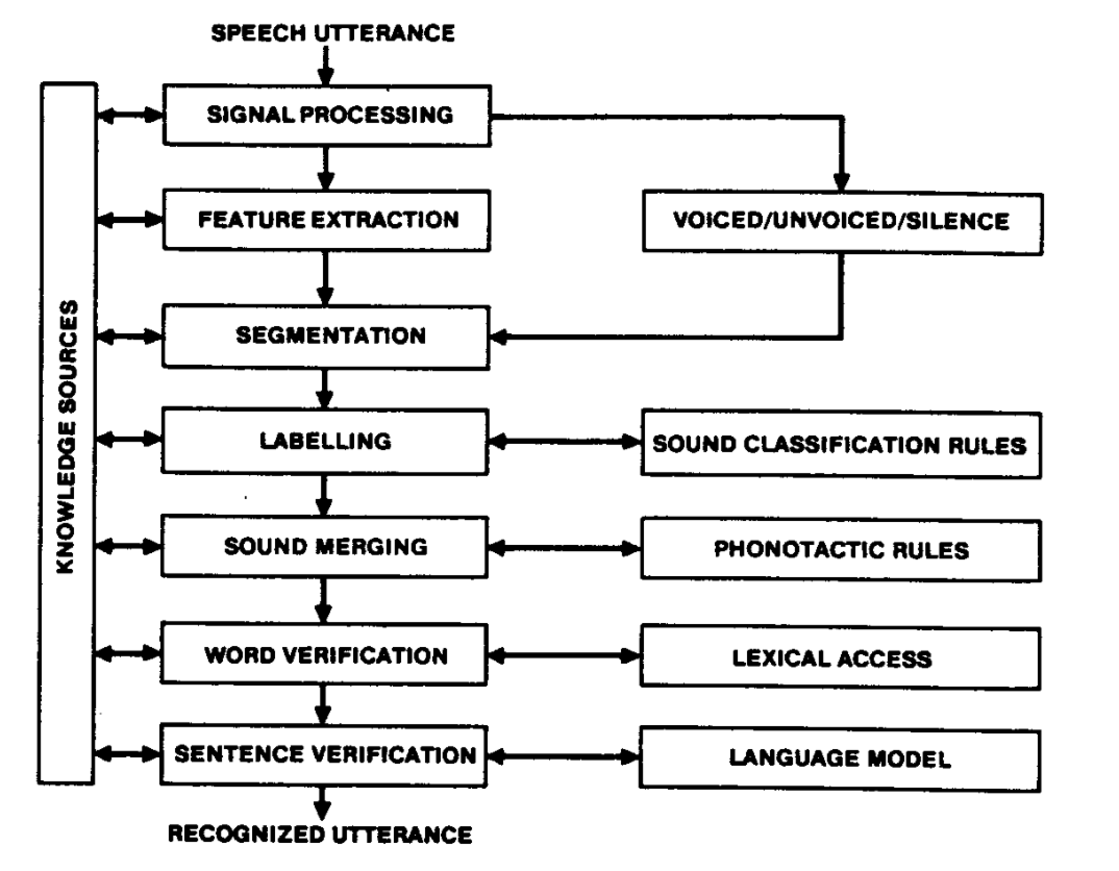
\includegraphics[width=0.7\textwidth]{stt_pipeline.pdf}
    \caption{Knowledge integration in speech recognition \cite{rabiner1993speechrecognition}}
    \label{fig:stt_pipeline}
\end{figure}

\section{Large Language Models}

% large language models, was ist, welche gibts, wieso chat gpt api??

